\section{Statechart Refinement}
\label{sec:refinement-rules}

The work presented here includes three refinement rules.
\begin{enumerate}
\item  \emph{Rule A:} Guard conditions on a transition can be strengthened (but not weakened); 
this can be done by adding textual guards to the transition, or
changing the source of the transition to a nested state.
\item \emph{Rule B:} Transitions can have additional actions, provided they do not
  modify variables appearing in the abstraction; this can be 
  accomplished by adding textual action to the transition 
  or by changing the target to nested state.
\item \emph{Rule C:} A state-chart can be embedded within a state of another
  state-chart -- sometimes called hierarchical composition or
  hierarchical refinement.
\end{enumerate}

The application of these rules is illustrated in figure~\ref{fig:ref-rules}.
\emph{Rule A} is applied to refine the abstract transition from |SA| to |SB| after adding 
child states |SC| and |SD|. The refinement strengthens the guard of the transition 
by restricting it to |SD|. On the other hand, \emph{Rule B} refines the abstraction 
by introducing a new concrete variable, $x$, into the model. The abstract transition is refined 
by the actions associated with this new variable. Finally \emph{Rule C} constructs a refinement 
introducing statecharts |SC, SD| and |SG, SH| through hierarchical and parallel composition respectively.

\begin{figure}[]
	\centering
	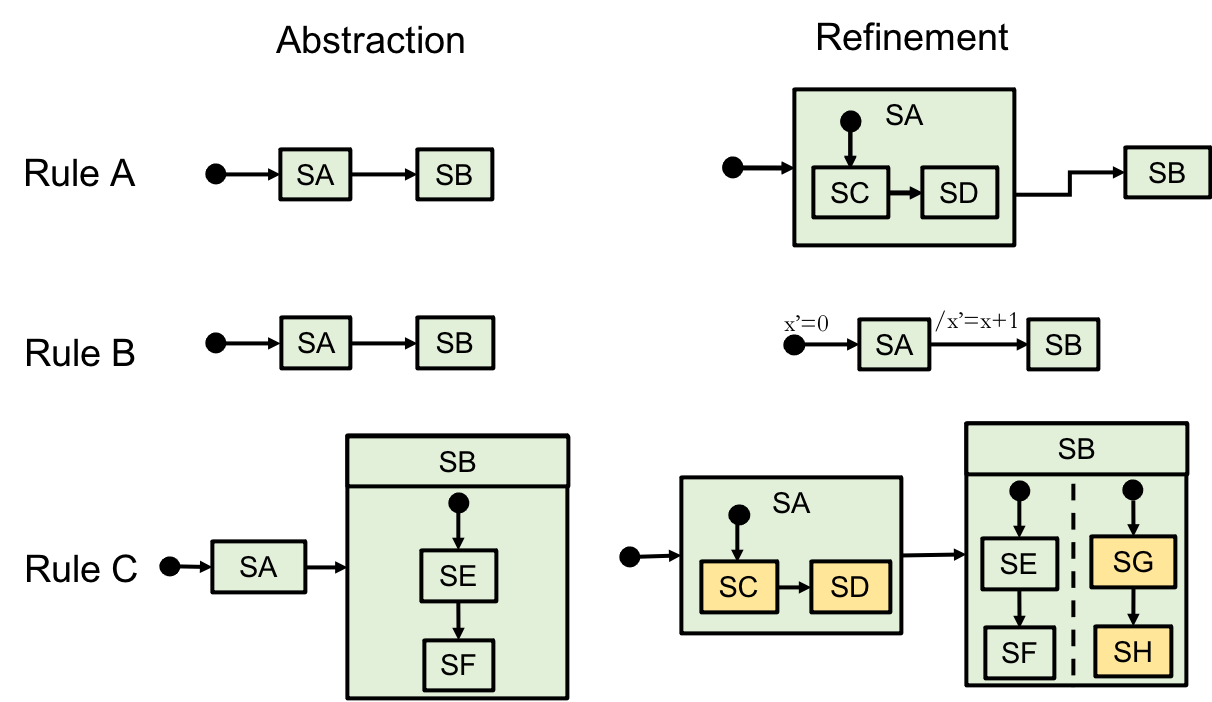
\includegraphics[width=0.90\textwidth]{figures/RefinementRules.png}
	\caption{Statechart refinement rules}
	\label{fig:ref-rules}
\end{figure} 

Via the translation explained in Section~\ref{sec:translation}, these
rules rely on the usual \EventB proof obligations to ensure that they
do indeed yield refinements in the \EventB semantics.